\documentclass[twocolumn,aps,prx,amsmath,amssymb,longbibliography,superscriptaddress]{revtex4-2}
\usepackage{graphicx}
\usepackage{dcolumn}
\usepackage{bm}
\usepackage{amsfonts}
\usepackage{xcolor,tabu}
\usepackage{multirow}
\usepackage{amsthm}
\usepackage{textcomp}
\usepackage{tikz}
\usepackage[colorlinks=true,
            linkcolor=blue,
            urlcolor=blue,
            citecolor=blue]{hyperref}
\hypersetup{bookmarksopen=true}
\usepackage{xr}
\usepackage{float}
\usepackage[normalem]{ulem}
% Comment type:
  % -- general comments and communications: questions, uncertainties, marks for further considerations, etc.
  %% -- the original sentence
  %%% -- my changes and reason(s) for the change

% modified sentences will be used in the main text.
% comments will be below the modified sentence

% Things to discuss:
% 1. Some words may be used too many times: systematic, surprising/unusual/unexpected/
\begin{document}

\title{Density Fluctuations and Energy Spectra of 3D Bacterial Suspensions}




\author{Zhengyang Liu}
\affiliation{Department of Chemical Engineering and Materials Science, University of Minnesota, Minneapolis, MN 55455, USA}
%\email{liux3141@umn.edu}
\author{Wei Zeng}
% \altaffiliation[Current address: ]{State Key Laboratory for Conservation and Utilization of Subtropical Agro-bioresources, Guangxi Microorganism and Enzyme Research Center of Engineering Technology, College of Life Science and Technology, Guangxi University, Nanning 530004, Guangxi, China.}
\affiliation{Department of Chemical Engineering and Materials Science, University of Minnesota, Minneapolis, MN 55455, USA}
\affiliation{College of Life Science and Technology, Guangxi University, Nanning 530004, Guangxi, China}
\author{Xiaolei Ma}
\author{Xiang Cheng}
\email{xcheng@umn.edu}


\affiliation{Department of Chemical Engineering and Materials Science, University of Minnesota, Minneapolis, MN 55455, USA}


\date{\today}


\begin{abstract}
We experimentally study density fluctuations and energy spectra of bulk \textit{E. coli} suspensions of different concentrations. Our results verify the predicted scaling law of giant number fluctuations in three-dimensional (3D) wet active fluids. Surprisingly, we find that such a scaling behavior persists at small scales even in low-concentration suspensions well below the transition concentration to active turbulence. Furthermore, our experiments also support the prediction on the energy spectra of dilute pusher swimmers and illustrate the spectral properties of the active turbulence of dense bacterial suspensions in the bulk limit. More importantly, we examine the density-energy coupling in both the steady and transient states of active turbulence. A universal density-independent and scale-invariant correlation between giant number fluctuations and energy spectra is uncovered across a wide range of length scales.

\end{abstract}

\maketitle

\section{introduction}

Active fluids exhibit many unusual behaviors beyond the expectation of equilibrium statistical mechanics \cite{Ramaswamy2010,Cates2012,Marchetti2013,Poon2013,Elgeti2015}.
In particular, an active fluid can exhibit anomalously large density variations, the so-called giant number fluctuations (GNF), where the standard deviation of the number of particles $\Delta N$ grows nonlinearly with the square root of the mean particle number $\sqrt N$, defying the central limit theorem of equilibrium systems \cite{Mishin2015}.
Such unusual density fluctuations have been observed in various active fluids in both living and non-living systems including vibrated granular rods \cite{Narayan2007,Aranson2008,Kudrolli2008,Deseigne2010}, swarming bacteria \cite{Zhang2010,Nishiguchi2017} and mammalian cells \cite{Kawaguchi2017},
self-propelled cytoskeleton \cite{Schaller2013}, and synthetic colloidal swimmers \cite{Palacci2013,Karani2019}. Hence, GNF is generally viewed as a hallmark of the emergent behaviors of active fluids.


Although significant progress has been made in the theoretical understanding of GNF over the past two decades \cite{Toner1995, Tu1998, Toner1998, AditiSimha2002, Ramaswamy2003, Toner2005, Chate2008, Mishra2010, Dey2012, Saintillan2012, Saintillan2013, Ngo2014,  Mahault2019}, systematic experiments that can quantitatively verify theoretical and numerical predictions are still few and far between. Particularly, the existing experiments on GNF all focused on dry two-dimensional (2D) or quasi-2D systems \cite{Narayan2007, Aranson2008, Kudrolli2008, Deseigne2010, Zhang2010, Schaller2013, Nishiguchi2017, Kawaguchi2017, Palacci2013}, where particle-boundary interactions strongly affect density fluctuations \cite{Marchetti2013}.
Such system-specific interactions lead to a variety of reported scaling behaviors of GNF, $\Delta N/\sqrt N \sim N^\alpha$, in 2D active fluids.
Scaling exponents $\alpha$ ranging between 0.13 and 0.5 have been found in different 2D experiments. In contrast, measurements of GNF in 3D wet active fluids, where hydrodynamics dominate the interparticle interactions and conserve the total momentum of systems, have not been achieved heretofore. Experimental verification of the prediction of GNF in 3D wet active fluids without the influence of system boundaries is still out of reach. Important questions such as how the long-ranged hydrodynamic interactions and the dimensionality of systems affect the density fluctuations of active fluids have not been properly addressed experimentally.

The rise of GNF in active fluids is usually accompanied by the transition to ordered phases with collective motions \cite{Ramaswamy2010,Marchetti2013}. For wet active fluids such as bacterial suspensions, these collective motions lead to large-scale coherent flows with intermittent vortices and jets, a phenomenon often referred to as active turbulence \cite{Wolgemuth2008,Ishikawa2011,Wensink2012,Dunkel2013a,Bratanov2015,Peng2016,Guo2018,Linkmann2019,Bardfalvy2019,Alert2020,Skultety2020,Peng2020}. Similar to GNF that manifests density fluctuations across different scales, the flow of active turbulence also exhibits scale-dependent structures. Imported from the study of classical turbulence, energy spectra are frequently used to quantify such scale-dependent structures in active turbulence \cite{Ishikawa2011,Wensink2012,Dunkel2013a,Giomi2015,Creppy2015,Patteson2018,Bardfalvy2019,Alert2020}. Nevertheless, current experimental studies of energy spectra were limited to active turbulence at high particle concentrations. A systematic measurement of energy spectra over a broad range of particle concentrations is still missing. More importantly, although both GNF and energy spectra quantify the scale-dependent dynamics of active fluids, the intrinsic connection between these two quantities across different scales has not been investigated.

%
\begin{figure}[t]
	\begin{center}
		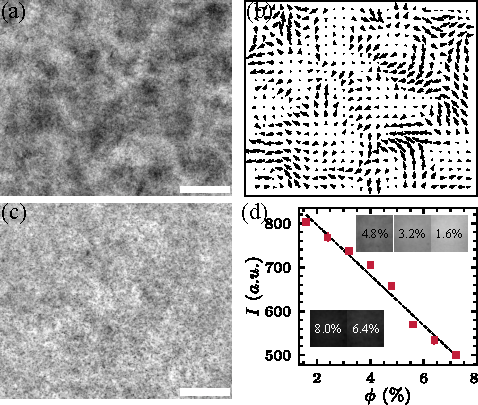
\includegraphics[width=0.46\textwidth]{Figures/fig-1.pdf}
		\caption[Experimental details]
		{Density fluctuations and active turbulence.
			(a) A snapshot of a dense suspension of \textit{E. coli} with bacterial volume fraction $\phi = 6.4\%$.
			(b) 2D velocity field of the suspension shown in (a), which exhibits characteristic active turbulent flow patterns.
			(c) A snapshot of a dilute suspension of \textit{E. coli} with $\phi = 1.6\%$, which shows no active turbulent flows. Scale bars are 85 $\mu$m.
			(d) Average pixel intensities of images, $I$, as a function of $\phi$. Inset shows the images of bacterial suspensions of different $\phi$ under the same light illumination.
		}
		\label{fig:experiment}
	\end{center}
\end{figure}




Here, we present our systematic experimental study of GNF and energy spectra of bulk bacterial suspensions, a premier example of 3D wet active fluids \cite{Marchetti2013}. First, our experiments on GNF in high-concentration bacterial suspensions quantitatively verify the theoretical prediction on the scaling behavior of density fluctuations in 3D wet active fluids. More surprisingly, we find that such a scaling relation persists at small scales even in low-concentration suspensions well below the transition concentration of active turbulence. Such an unusual behavior arises due to the long-range nature of hydrodynamic interactions, lacking in 2D dry systems. Second, our measurements on the energy spectra of bacterial suspensions of different concentrations further illustrate the emergence of the characteristic flow structure of active turbulence and confirm the prediction of the energy spectra of dilute pusher suspensions. Lastly, our experiments reveal a density-independent and scale-invariant coupling between GNF and energy spectra across a wide range of length scales. Quantitatively similar coupling has also been uncovered in the kinetic process during the transition towards active turbulence. Taken together, our study provides not only experimental verification of several important theoretical predictions including the scaling law of GNF in 3D wet active fluids, the energy spectra of dilute pusher swimmers and the delayed onset of density fluctuations, but also new insights into the emergent dynamics of bulk bacterial suspensions such as local swimmer correlations in dilute suspensions and the universal coupling between density fluctuations and flow energies.

\section{Experiment}

We use a genetically engineered light-powered \textit{Escherichia coli} (\textit{E. coli}) strain as our model active particles (Appendix~\ref{appendix-MM}).
In a typical experiment, a bacterial suspension of control volume fraction $\phi$ is injected into a sealed chamber of 20 mm $\times$ 3 mm $\times$ 140 $\mu$m. Here, we calculate $\phi = n V_b$, where $n$ is the number density of bacteria and $V_b$ is the volume of a single bacterium. We estimate $V_b = \pi (w_b/2)^2 l_b \approx 1$ $\mu$m$^3$ with $l_b = 3$ $\mu$m and $w_b = 0.65$ $\mu$m as the average length and width of a bacterial body. Without external oxygen supply, bacteria quickly consume all the oxygen in the chamber and stop moving after $5$ minutes.
We then illuminate the suspension using a high-intensity light, which powers bacteria at their maximal swimming speed of $v_0 = 15 \pm 3$ $\mu$m/s. A video of the suspension is taken 50 $\mu$m above the bottom wall of the chamber by a bright-field inverted microscope at a frame rate of $30$ fps with the field of view of $420 \times 360$ $\mu$m$^2$ (Fig.~\ref{fig:experiment}a).
We use a standard Particle Image Velocimetry (PIV) algorithm
to extract the 2D in-plane velocity field $\bm{v} = (v_x,v_y)$ in the 3D suspension (Appendix~\ref{appendix-IA-PIV}). The suspension exhibits the characteristic vortices and jets of active turbulence at high $\phi$ (Fig.~\ref{fig:experiment}b).

It is challenging to directly count the number of bacteria in a 3D dense suspension of fast moving bacteria. Luckily, by virtue of Beer-Lambert law, the local bacterial density is monotonically correlated with the local intensity of microscope images, where darker regions correspond to higher bacterial densities (Fig.~\ref{fig:experiment}a, c and Supplementary Video). Such a principle has been exploited in previous experiments in probing the dynamics of bacterial suspensions and actin filaments \cite{Sokolov2009, Wilson2011, Schaller2013}. To calibrate the density-intensity correlation, we prepare bacterial suspensions of different $\phi$ and image the suspensions under the same illumination (Fig.~\ref{fig:experiment}d inset). The mean image intensity decreases with increasing $\phi$ following an approximately linear relation (Fig.~\ref{fig:experiment}d), agreeing with the the Beer-Lambert law for samples of small thickness and weak absorptivity appropriate for our experiments. The linear density-intensity relation has also been used in previous studies to characterize the dynamics of \textit{E. coli} suspensions \cite{Wilson2011}.

\begin{figure}[t]
	\begin{center}
		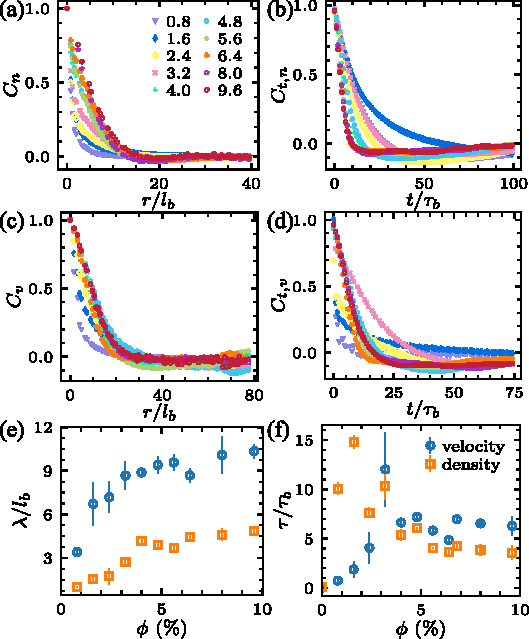
\includegraphics[width=0.46\textwidth]{Figures/fig-2.pdf}
		\caption[spatiotemporal-correlations.]
		{
			Density and velocity spatiotemporal correlations. (a) Two-point density correlations at different bacterial volume fractions $\phi$. Radial position $r$ is normalized by the average length of bacteria $l_b = 3$ $\mu$m. (b) Density autocorrelations at different $\phi$. Time $t$ is normalized by the characteristic swimming time of bacteria $\tau_b = 0.2$ s. (c) Two-point velocity correlations at different $\phi$. (d) Velocity autocorrelations at different $\phi$. $\phi$ ($\%$) of different curves are indicated in (a). (e) Density and velocity correlation lengths, $\lambda$, versus $\phi$. (f) Density and velocity correlation times, $\tau$, versus $\phi$. The error bars in (e) and (f) represent the standard deviations of measurements over 3 independent experiments.
		}
		\label{fig:spatiotemporal-correlations}
	\end{center}
\end{figure}




\section{Results}

\subsection{Density fluctuations}

The simple linear relation allows us to measure the spatiotemporal patterns of local bacterial densities and investigate density fluctuations in 3D bacterial suspensions. We first calculate the two-point density spatial correlation, $C_n$, and the density auto-correlation, $C_{t,n}$, for suspensions of different $\phi$ (Fig.~\ref{fig:spatiotemporal-correlations}a, b) and compare them with the well-studied velocity spatiotemporal correlations, $C_{v}$ and $C_{t,v}$, extracted from PIV (Fig.~\ref{fig:spatiotemporal-correlations}c, d).


\begin{figure}[t]
	\begin{center}
		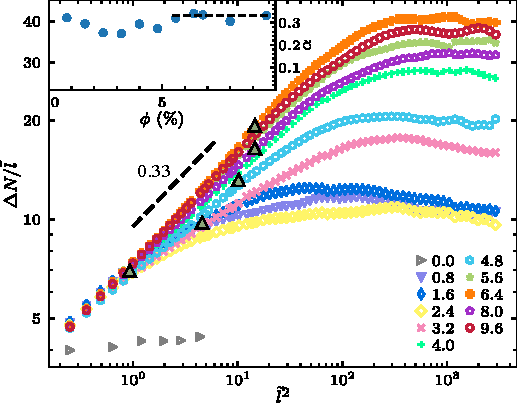
\includegraphics[width=0.47\textwidth]{Figures/fig-3.pdf}
		\caption[Concentration dependence of GNF.]
		{
			Density fluctuations of bacterial suspensions of different volume fractions $\phi$. The standard deviation of bacterial number $\Delta N$ in a subsystem of length $l$ as a function of the area of the subsystem $l^2$. $\Delta N$ is normalized by the length of the subsystem $l$, which is proportional to the square root of bacterial number in the subsystem $\sqrt N$. $l$ is presented in a dimensionless form, $\tilde{l} = l/l_b$, where $l_b = 3$ $\mu$m is the average length of bacteria. Dark green triangles indicate the density correlation lengths $\lambda(\phi)$ from Fig.~\ref{fig:spatiotemporal-correlations}e. The black dashed line indicates a power-law scaling of 0.33.
			Inset: Scaling exponent $\alpha$ versus $\phi$. $\alpha$ are extracted by fitting the experimental data from 0.3$l_b$ to $\lambda(\phi)$. The dashed line in the inset indicates the theoretical prediction of $\alpha=1/3$.
		}
		\label{fig:GNF}
	\end{center}
\end{figure}

The correlation length $\lambda$ and correlation time $\tau$ are determined when the corresponding normalized correlation functions decay to $1/e$. Figure~\ref{fig:spatiotemporal-correlations}e shows the density correlation length $\lambda$ at different $\phi$, which quantifies the scale of density inhomogeneities in suspensions.
$\lambda$ is small at low $\phi$, gradually increases with $\phi$ and reaches a plateau of $\sim 5l_b$ in high-concentration bacterial suspensions when $\phi > \phi_c$. Here, $\phi_c = 3.2\%$ is the transition concentration above which suspensions show active turbulence \cite{Peng2020}.
% \textcolor{red}{Is $\phi_c$ the transition concentration to active turbulence?}
The velocity correlation length follows a qualitatively similar trend and also saturates above $\phi_c$, consistent with previous findings \cite{Sokolov2007}. The saturated velocity correlation length is about twice of the saturated density correlation length, which is determined by the size of system \cite{Guo2018}.  Figure~\ref{fig:spatiotemporal-correlations}f further compares the density and velocity correlation times, $\tau$, at different $\phi$. Although the density and velocity correlation times at low $\phi$ show a large discrepancy, they both plateau when $\phi > \phi_c$ around $5\tau_b$, where $\tau_b=l_b/v_0=0.2$ s is the characteristic swimming time scale of \textit{E. coli}. The saturated velocity correlation time is slightly larger than the saturated density correlation time. The similarity between the density and the velocity correlation functions at high $\phi$ indicates a strong coupling between density fluctuations and active turbulent flows, a feature we shall
examine in more details in Sec.~\ref{Density-flow coupling}.


We further examine GNF by calculating the standard deviation of bacterial number $\Delta N$ for subsystems of different sizes (Appendix~\ref{sec:GNF-calculations}). Figure~\ref{fig:GNF} shows $\Delta N$ as a function of the area of subsystems $l^2$ for bacterial suspensions of different $\phi$, where $l$ is the side length of square subsystems. Note that since the depth of field of our images $d$ is fixed, the volume of subsystems is $l^2 d$, which gives $N = l^2d \phi/V_b$. Thus, the average number of bacteria in subsystems $N$ is linearly proportional to $l^2$ at a fixed $\phi$. To highlight the deviation of the scaling from the central limit theorem, we normalize $\Delta N$ by $l \sim \sqrt N$ in the figure.

At a given $\phi$, $\Delta N/l$ plateaus following the central limit theorem when $l$ is significantly larger than the density correlation length at the corresponding $\phi$, $\lambda(\phi)$ (Fig.~\ref{fig:spatiotemporal-correlations}e). The central limit theorem applies at large length scales owing to the spatial average over multiple dense and dilute regions. Nevertheless, at small length scales when $l$ is comparable or smaller than $\lambda(\phi)$, bacterial suspensions of all $\phi$ in our study exhibit obvious GNF, where $\Delta N/l$ increases with increasing subsystem size. Remarkably, $\Delta N/l$ versus $l^2$ converges to the same scaling in the small $l$ limit even for low-$\phi$ suspensions without turbulent flows. Such a surprising finding is in direct contrast to GNF of 2D active systems, where GNF diminishes with decreasing particle concentrations and disappears for low-concentration samples \cite{Narayan2007,Aranson2008,Kudrolli2008,Deseigne2010,Zhang2010,Schaller2013}. Kinetic theories have predicted that, due to the long-range hydrodynamic interactions, pusher-type microswimmers in 3D active suspensions show strong spatial and temporal correlations at low concentrations well below the transition concentration to active turbulence \cite{Stenhammar2017,Nambiar2021}. Although the theories only discussed the effect of the correlation on the enhanced diffusion of passive tracers and velocity fluctuations in dilute suspensions, our experiments show that such a correlation also manifests as GNF at small length scales in low-concentration bacterial suspensions.


Quantitatively, the strength of GNF can be measured by the scaling exponent $\alpha$ following $\Delta N/\sqrt{N} \sim N^\alpha$. $\alpha=0$ for equilibrium systems obeying the central limit theorem, whereas the upper bound $\alpha = 0.5$ corresponds to a system with maximal density fluctuations.
We extract $\alpha$ by fitting the experimental curves with the power-law relation for $l < \lambda(\phi)$. The inset of Fig.~\ref{fig:GNF} shows $\alpha$ as a function of $\phi$, where $\alpha$ remains approximately constant at $0.30 \pm 0.03$ for all $\phi$. In contrast, $\alpha$ decreases with decreasing $\phi$ for 2D GNF. Notably, for high $\phi \geq 5.6\%$, $\alpha$ stabilizes to $0.33 \pm 0.01$, quantitatively agreeing with the theoretical prediction of $\alpha = 1/3$ for 3D suspensions of polar-ordered self-propelled particles with hydrodynamic interactions \cite{AditiSimha2002}. Hence, our experiments for the first time quantitatively verify the theory of the GNF of 3D wet active fluids. More interestingly, our study shows that the same GNF scaling persists in low-concentration suspensions at small scales even before the emergence of the large-scale orientational order discussed in the theory.

\begin{figure}[t]
\begin{center}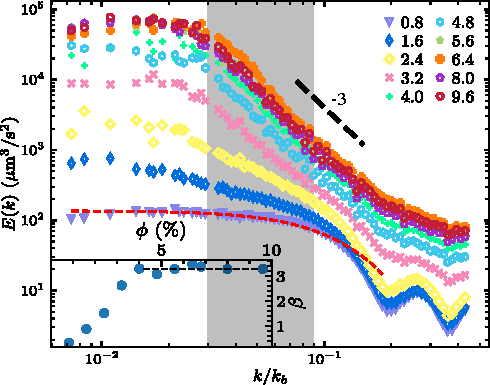
\includegraphics[width=0.47\textwidth]{Figures/fig-4.pdf}
\caption[Concentration dependence of energy spectra.]
{
Energy spectra $E(k)$ of bacterial suspensions of different volume fractions $\phi$. Shaded region indicates the range over which the scaling exponent $\beta$ is fitted. The black dashed line indicates a power-law scaling of $-3$. The red dashed line is a fitting of $E(k)$ at $\phi=0.8\%$ using Eq.~\ref{eq:energy-spectra}. In the fitting, the bacterial number density $n=\phi V_b$ and the dipole length $l_d = 1.9$ $\mu$m are from experiments, whereas the dipole strength $\kappa = 100$ $\mu$m$^3$/s and the regularization length $\epsilon = 14$ $\mu$m are taken as fitting parameters. In comparison, $\kappa = 300.8$ $\mu$m$^3$/s from experiments (see text).
Inset: Scaling exponent of $E(k)$, $\beta$, as a function of $\phi$. Dashed line indicates $\beta = 3.3$.
% \textcolor{red}{}.
}
\label{fig:energy-spectra}
\end{center}
\end{figure}

\subsection{Energy spectra}

Similar to GNF, the velocity field of active turbulence also shows scale-dependent structures, which are often characterized by the energy spectrum of turbulent flows, $E(k)$ (Appendix~\ref{appendix-IA-ES}). $E(k)$ measures the kinetic energy density at different scales in terms of wavenumber $k = 2\pi/l$. It is related to the mean kinetic energy density by $\langle \bm{v}^2 \rangle/2 = \langle v_x^2 + v_y^2 \rangle/2 = \int_0^\infty E(k)dk$. Figure~\ref{fig:energy-spectra} shows $E(k)$ of bacterial suspensions at different $\phi$. In the dilute suspension of $\phi = 0.8 \%$, $E(k)$ is independent of $k$ in the small $k$ limit and then decreases at high $k$. The oscillation observed at high $k$ likely arises from PIV errors due to the small number of bacteria in each PIV box of low-$\phi$ suspensions. With increasing $\phi$, $E(k)$ at small $k$ increases sharply. In the turbulent regime at high $\phi$, the kinetic energy is concentrated at scales much larger than the size of single bacteria, even though the turbulent flow is entirely driven by the swimming of single bacteria. The overall trend of $E(k)$ with increasing $\phi$ qualitatively agrees with the results from large-scale particle simulations \cite{Saintillan2012,Bardfalvy2019}.


$E(k)$ of low-$\phi$ suspensions with uncorrelated pusher swimmers has been predicted \cite{Bardfalvy2019}
\begin{equation}
\label{eq:energy-spectra}
E(k) = 4\pi n \kappa^2 \left[ \frac{1}{3} + \frac{\cos(kl_d)}{(kl_d)^2} - \frac{\sin(kl_d)}{(kl_d)^3} \right] \frac{\epsilon^4k^2}{l_d^2} K_2^2(k\epsilon),
\end{equation}
where $n$ is the number density of bacteria, $\kappa$ is the dipole strength and $l_d$ is the dipolar length of \textit{E. coli}. $\epsilon$ is the distance for the regularization of the dipolar flow field. $K_2$ is the modified Bessel function of the second kind.
The fitting of Eq.~\ref{eq:energy-spectra} agrees well with our experimental $E(k)$ at low $\phi$ in the small $k$ limit (Fig.~\ref{fig:energy-spectra}). Particularly, Eq.~\ref{eq:energy-spectra} dictates that $E(k)$ is flat as $k \to 0$, a key feature confirmed by our experiments. A simple dimensional analysis can show that the plateau $E(k)$ at the small $k$ follows $\lim_{k \to 0}E(k) \sim n \kappa^2$ for uncorrelated swimmers of density $n$. The dipole strength can be estimated as $\kappa = Fl_d/\eta = \xi v_0 l_d/\eta = 300.8$ $\mu$m$^3$/s, where $\eta$ is the viscosity of the buffer. $\xi$ is the drag coefficient of a bacterial body orientated along its major axis, which can be calculated based on the body geometry $\xi = 3\pi\eta w_b \left[1-(1-l_b/w_b)/5\right]$ \cite{Magariyama2002}. $l_d = 1.9$ $\mu$m is taken from direct measurements \cite{Drescher2011}. Thus, $\lim_{k \to 0}E(k) \approx 7 \times 10^2$ $\mu$m$^3$/s, within the same order of magnitude of our experiments. The discrepancy between Eq.~\ref{eq:energy-spectra} and experiments at large $k$ may arise from the strong bacterial correlation at small length scales as shown by density fluctuations as well as the PIV errors.


We also extract the scaling exponent $\beta$ of $E(k) \sim k^{-\beta}$ by fitting the energy spectra at intermediate $k$, where a significant change of $E(k)$ with $\phi$ occurs and $E(k)$ exhibits good power-law relations. $\beta$ increases with $\phi$ and saturates around 3 at high $\phi > \phi_c$ (Fig.~\ref{fig:energy-spectra} inset). The saturated scaling exponent quantitatively agrees with previous experimental results obtained from the active turbulence of high-concentration sperm suspensions and \textit{B. subtilis} suspensions at large $k$ \cite{Creppy2015, Wensink2012}. At small $k$, $E(k)$ reported in Ref.~\cite{Wensink2012} decreases with decreasing $k$ and exhibits a non-monotonic trend, different from the result in this work. Such discrepancy is attributed to the confined geometry used in \cite{Wensink2012}, which limits the size of turbulent vortices and thus leads to a decrease of $E(k)$ at small $k$ \cite{Guo2018}. The large system size of $L = 140$ $\mu$m of our experiments allows us to probe the small $k$ limit predicted by theories and simulations without the influence of system boundaries.

Although the scaling in the small $k$ limit is strongly affected by the system size, the scaling in the large $k$ limit seems to be universal with $\beta \approx 3$ from different experiments. To the best of our knowledge, no theoretical prediction has been made on this universal scaling behavior for 3D active turbulence. Giomi investigated the energy spectra of 2D active nematics by combining numerical simulations with mean-field theories and showed $E(k) \sim k^{-4}$ in the large $k$ limit \cite{Giomi2015}.
The result has also been confirmed recently by a hydrodynamic theory \cite{Alert2020}. For isotropic turbulence in $d$ dimension, the energy spectra can be written as $E(k) = C_d k^{d-1} \langle \mathbf{v}(\mathbf{k})\cdot \mathbf{v}(-\mathbf{k})\rangle_{k = |\mathbf{k}|}$ \cite{Wensink2012,Bardfalvy2019},
where $C_d k^{d-1}$ is the surface area of $(d-1)$-sphere and $\langle \mathbf{v}(\mathbf{k})\cdot \mathbf{v}(-\mathbf{k})\rangle_{k = |\mathbf{k}|}$ is the Fourier transform of the velocity-velocity spatial correlation function. If the velocity correlation function for 2D active nematics is qualitatively similar to that of 3D bacterial suspensions independent of the dimensionality of systems, the mean-field theory would then predict a scaling of $E(k) \sim k^{-3}$, consistent with experimental observations. Such a hypothesis, although intriguing, is certainly non-trivial and needs further theoretical investigation.

\begin{figure}[t]
\begin{center}
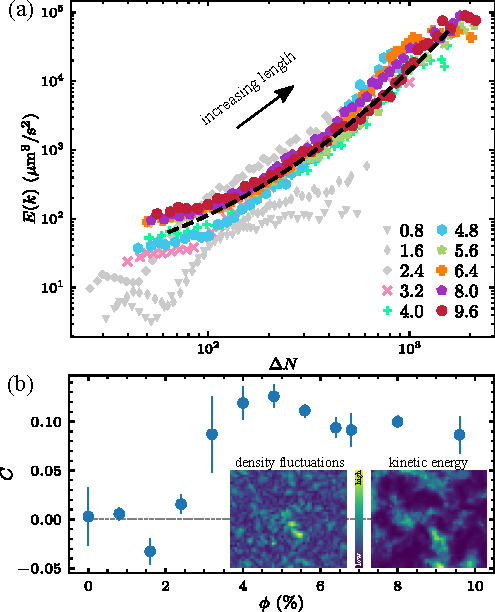
\includegraphics[width=0.47\textwidth]{Figures/fig-5.pdf}
\caption[The correlation between GNF and kinetic energy and kinetic energy spectra.]
{
Coupling between density fluctuations and kinetic energies in the steady state.
(a) Energy spectra $E(k)$ plotted against number density fluctuations $\Delta N$ at each corresponding length scale for bacterial suspensions of different volume fractions $\phi$. Gray symbols are used for low-$\phi$ suspensions without active turbulence. The black dashed line is a polynomial fitting of the master curve, serving as guide for the eye. The black arrow indicates the direction of increasing lengths.
(b) Correlation of local density fluctuations and kinetic energies $C$ as a function of $\phi$. $C$ is averaged over 1000 frames in steady state, and the error bars represent the standard deviations (see Appendix.~\ref{appendix-IA-localcorrelation}) Inset: Density fluctuation and kinetic energy fields in a bacterial suspension of $\phi = 4.8\%$.
}
\label{fig:GNF-energy-spectra-correlation}
\end{center}
\end{figure}

\subsection{Density-energy coupling} \label{Density-flow coupling}

\begin{figure*}[t]
\begin{center}
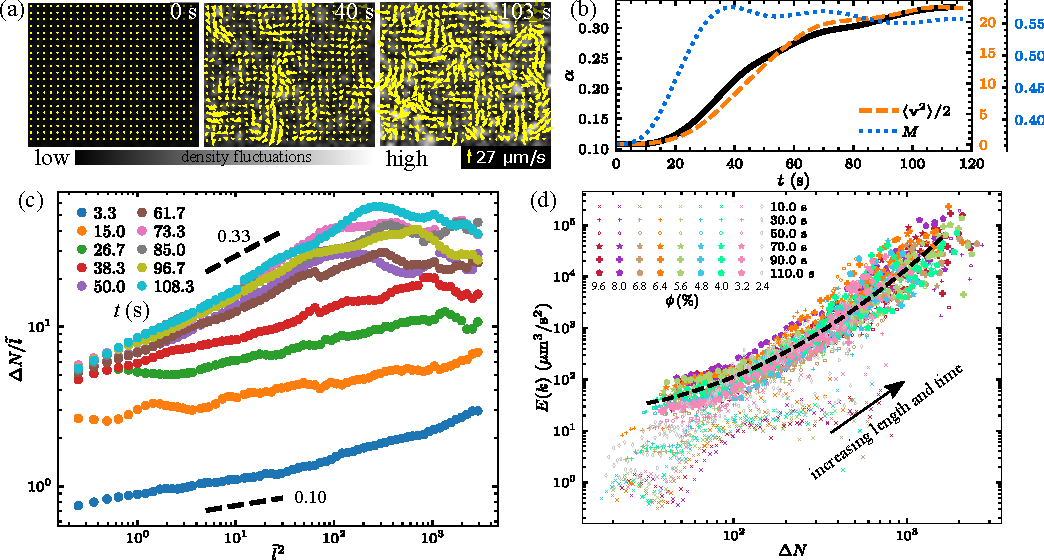
\includegraphics[width=0.89\textwidth]{Figures/fig-6.pdf}
\caption[The correlation between GNF and kinetic energy and kinetic energy spectra at transient state]
{
Density-energy coupling in the transient state during the transition towards active turbulence.
(a) The field of density fluctuations and the velocity field of a bacterial suspension of volume fraction $\phi=6.4\%$ at different time $t$ in the transient state. The gray-scale background indicates the magnitude of local density fluctuations (see Appendix~\ref{appendix-IA-localcorrelation}), whereas the yellow arrows show the local velocities. Light is turned on at time $t = 0$.
(b) Temporal evolution of the GNF scaling exponent $\alpha$, the total kinetic energy $\langle \bm{v}^2 \rangle/2$ and the area fraction of regions with collective flow $M$ from the same transition shown in (a).
(c) Number density fluctuations $\Delta N$ as a function of subsystem size $l^2$ at different times over the turbulence transition of the same bacterial suspension shown in (a). $\Delta N$ is normalized by the length of subsystems $l$, similar to that in Fig.~\ref{fig:GNF}. $\tilde{l} = l/l_b$. $t$ is indicated in the legend.
(d) Energy spectra $E(k)$ versus density fluctuations $\Delta N$ during the active turbulent transition. $t$ and $\phi$ are encoded in the marker size and color, respectively. The black dashed line is the fitting of the master curve shown in Fig.~\ref{fig:GNF-energy-spectra-correlation}a.
}
\label{fig:GNF-energy-spectra-correlation-transient}
\end{center}
\end{figure*}

Both GNF and energy spectra probe the scale-dependent properties of active bacterial suspensions. While the former measures density fluctuations at different scales, the latter considers the transfer of flow energies % Aranson2007 PRE
across scales. Although both quantities have been extensively studied separately, a direct correlation between the two has not been explicitly examined heretofore. Indeed, the quantitative similarity between the density spatiotemporal correlations and the velocity spatiotemporal correlations shown in Fig.~\ref{fig:spatiotemporal-correlations} has already indicated a strong coupling between density fluctuations and active turbulent flows in the turbulent regime. Moreover, the trends of GNF and energy spectra also show similar characteristics, both exhibiting a rapid increase at small length scales and plateaus at large length scales (Figs.~\ref{fig:GNF} and \ref{fig:energy-spectra}). Such a similarity suggests that a density-independent correlation between density fluctuations and kinetic energies may exist across different length scales. To verify the hypothesis, we plot density fluctuations $\Delta N$ against the corresponding kinetic energy densities $E(k)$ at the same scale in Fig.~\ref{fig:GNF-energy-spectra-correlation}a. We find that all the $\Delta N$-$E$ pairs in the turbulent regime fall onto a master curve over a wide range of length scales extending from the size of a single PIV step ($\sim 8$ $\mu$m) up to the size of the entire system ($> 140$ $\mu$m), regardless of the volume fractions of the samples.
In contrast, $\Delta N$-$E$ shows much stronger scattering for low $\phi$ suspensions without active turbulence. Although it is not surprising that density fluctuations should correlate with kinetic energies in general as both measure different aspects of the same active turbulence, the collapse of data from samples of different volume fractions is still quite unexpected.
The result shows that the coupling between density fluctuations and turbulent flows occurs at every scale of active turbulence in a quantitative same fashion. Such a scale-invariant coupling is independent of the volume fraction of bacterial suspensions.



To illustrate such an unusual coupling in real space, we calculate the correlation of \emph{local} density fluctuations and kinetic energies at the smallest length scale of our PIV analysis, i.e., the step size of PIV at $l = 2.75l_b$. The local density fluctuation $\delta N(\bm{r},t)$ and local kinetic energy $E(\bm{r},t)$ at position $\bm{r} = (x,y)$ and time $t$ are extracted from the image intensity field and the PIV velocity field, respectively (Fig.~\ref{fig:GNF-energy-spectra-correlation}b inset) (Appendix~\ref{appendix-IA-localcorrelation}).
The normalized correlation between $\delta N(\bm{r},t)$ and $E(\bm{r},t)$ averaged over all $\bm{r}$ and $t$ is then computed at different $\phi$ (Fig.~\ref{fig:GNF-energy-spectra-correlation}b). At low $\phi$ without active turbulence, the correlation is weak and fluctuates around zero, which then increases sharply with $\phi$ as the bacterial suspensions transition to active turbulence. A constant positive correlation is found in the turbulent regime when $\phi > \phi_c$. This real-space correlation provides a concrete example of the coupling between density fluctuations and turbulent kinetic energies at small scales.



More surprisingly, we find that the same density-energy coupling also exists in the kinetic process during the transition towards bacterial turbulence. Taking the advantage of the light-powered bacteria, we trigger the onset of bacterial turbulence by suddenly turning on the light illumination on high-$\phi$ bacterial suspensions at $t=0$ \cite{Peng2020}.
The temporal evolution of density fluctuations and turbulent flows in a bacterial suspension of $\phi = 6.4\%$ during the kinetic process is illustrated in Fig.~\ref{fig:GNF-energy-spectra-correlation-transient}a.
At $t=0$, the flow velocities are close to 0. The suspension shows no sign of density fluctuations. At $t=40$ s, although the magnitudes of velocities are still small, local alignment of velocity directions can be clearly observed, which gives rise to the characteristic pattern of vortices and jets of active turbulence. Weak density fluctuations start to emerge. At $t=103$ s, the magnitudes of velocities grow significantly and saturate. The suspension reaches the steady state of active turbulence with strong density fluctuations. Note that the response time of individual bacteria is much shorter than the emergence of collective flows. A single bacterium recovers its swimming speed within a few seconds after turning on the light \cite{Peng2020}.

Quantitatively, we monitor the temporal evolution of density fluctuations and energy spectra of the suspension in the transient state before the suspension reaches the steady turbulence (Appendix~\ref{appendix-IA-transient}). Figure ~\ref{fig:GNF-energy-spectra-correlation-transient}c shows the growth of GNF during the turbulent transition. Different from the steady-state GNF at different $\phi$, where strong GNF persists at small length scales even for low-$\phi$ suspensions, the high-$\phi$ bacterial suspension shows no or very weak GNF at the onset of active turbulence near $t=0$, with a small scaling exponent $\alpha \approx 0.10$ at early times. The strength of GNF, quantified by $\alpha$, gradually increases over time (the black line in Fig.~\ref{fig:GNF-energy-spectra-correlation-transient}b). $\alpha$ saturates to the steady state value of 0.33 above $t \approx 90$ s. Interestingly, the growth of GNF is significantly delayed compared with the formation of collective turbulent flows, which is measured by the area fraction of the regions with strong local velocity alignment, $M$ \cite{Cisneros2011, Peng2020}. $M$ reaches a plateau at a much earlier time around 30 s (the blue dotted line in Fig.~\ref{fig:GNF-energy-spectra-correlation-transient}b). The finding provides strong experimental evidence to an important prediction of the kinetic theory of active fluids \cite{Saintillan2008a, Saintillan2008b}, where density fluctuations are shown to be the consequence of the nonlinear development of the hydrodynamic instability of pusher swimmers and appear only at long times. In the linear regime, at the onset of the hydrodynamic instability with the initial rise of the collective turbulent flow, density fluctuations remain weak. While $\alpha$ and $M$ show a clear separation of time scales, we find that the growths of $\alpha$ and the kinetic energy $E$ are strongly coupled and exhibit quantitatively similar trends in the transient state (the black and the orange lines in Fig.~\ref{fig:GNF-energy-spectra-correlation-transient}b). The observation unambiguously demonstrates the density-energy coupling in the kinetic process.

Finally, we also analyze the correlation between GNF $\Delta N$ and energy spectra $E(k)$ during the turbulent transition for bacterial suspensions of different $\phi$ (Fig.~\ref{fig:GNF-energy-spectra-correlation-transient}d). When $\phi>\phi_c$, all our data at different $\phi$ and $l$, as well as at different $t$ except for the earliest time of 10 s close to the biological light response time of bacteria (``x'' markers in Fig.~\ref{fig:GNF-energy-spectra-correlation-transient}d), collapse into the same master curve obtained from the steady-state measurements.
The result suggests that kinetic energies control not only the steady-state GNF but also the rise of GNF at each individual length scale.

\section{Conclusions}

We have conducted systematic experiments measuring density fluctuations and energy spectra of 3D bacterial suspensions over a wide range of concentrations in both steady and transient states. We illustrated the scaling behavior of giant number fluctuations in bulk bacterial suspensions and showed that such a scaling persisted at small scales even in low-concentration suspensions well before the transition to active turbulence. The finding provided new experimental evidence on the existence of local spatial and temporal correlations between bacteria in dilute suspensions due to the long-range hydrodynamic interactions unique to 3D wet active fluids. In addition, we also examined the energy spectra of bacterial suspensions of different concentrations and showed the spectral properties of the active turbulence of dense bacterial suspensions in the bulk limit. Lastly, by comparing density fluctuations and energy spectra at different scales, we revealed an unexpected coupling between density fluctuations and kinetic energies across more than one order of magnitude of length scales from the scale of single bacteria up to the size of the system. We further showed that such a density-independent and scale-invariant coupling also dominated the kinetic process during the transition towards bacterial active turbulence.

Our experiments also verified several important theoretical predictions on 3D wet active fluids:

1) The scaling behavior of density fluctuations observed in our experiments, $\Delta N/\sqrt N \sim N^{0.33}$, quantitatively agreed with the theoretical prediction on the giant number fluctuations of 3D suspensions of polar-ordered self-propelled particles \cite{AditiSimha2002}.

2) The energy spectra of low-concentration bacterial suspensions measured in our study confirmed the key feature of the predicted energy spectra of uncorrelated pusher swimmers in the small wavenumber limit \cite{Bardfalvy2019}.

3) The delayed onset of density fluctuations uncovered in our experiments supported the central prediction of the kinetic theories on the nonlinear development of the hydrodynamic instability of pusher suspensions \cite{Saintillan2008a, Saintillan2008b}.

Thus, our study provided a comprehensive experimental benchmark on the density fluctuations and energy spectra of bulk bacterial suspensions and shed new light onto the emergent dynamics of 3D wet active fluids.


\begin{acknowledgements}
	We thank D. Ghosh, Y. Peng, Y. Qiao and K. Zhang for the help with experiments and fruitful discussions. The research is supported by NSF CBET 1702352, NSF CBET 2028652 and the Packard foundation.
\end{acknowledgements}

\appendix
\section{Materials and methods} \label{appendix-MM}
\subsection{Light-powered \textit{E. coli}}
We introduce a light-driven transmembrane proton pump, proteorhodopsin (PR), to wild-type \textit{E. coli} (BW25113) by transforming the bacteria with plasmid pZE-PR encoding the SAR86 $\gamma$-proteobacterial PR-variant \cite{Walter2007}. The activity of PR is correlated with the intensity of light. Thus, we can control the swimming speed of bacteria using light of different intensities. In our experiments, we use high-intensity light, which saturates the light response of bacteria. The average swimming speed of bacteria is fixed at $v_0 = 15 \pm 3$ $\mu$m/s.

The bacteria are cultured at 37 \textcelsius{} with a shaking speed at 250 rpm for 14-16 hours in terrific broth (TB) [tryptone 1.2\% (w/w), yeast extract 2.4\% (w/w), and glycerol 0.4\% (w/w)] supplemented with 0.1 g/L ampicillin. The culture is then diluted 1:100 (v:v) in fresh TB and grown at 30 \textcelsius{} for 6.5 hours. PR expression is triggered by supplementing the culture medium with 1 mM isopropyl $\beta$-D-thiogalactoside and 10  $\mu$M ethanolic all-trans-retinal in the mid-log phase, 3 hours after the dilution.

The bacteria are harvested by gentle centrifugation ($800g$ for 5 min). After discarding the culture medium in the supernatant, we resuspend bacteria with DI water. The resuspended suspension is then centrifuged again at $800g$ for 5 min, and finally adjusted to the target concentration for experiments.

\subsection{Sample preparation and microscopy}

To prepare the sample for microscopy, we construct a seal chamber made of glass slides (25 mm $\times$ 75 mm) and coverslips (18 mm $\times$ 18 mm). We first glue (NOA 81, Norland, NJ) two coverslips on a glass slide, side-by-side, leaving a 3-mm separation between the two coverslips. We then cover the 3-mm separation with another coverslip to form a channel. We pipette bacterial suspensions into the channel. Finally, the two ends of the channel are sealed by UV glue (NOA 76, Norland, NJ) to form a sealed chamber.

Images of the bacterial suspensions are taken 50 $\mu$m above the bottom surface of the sealed chamber by a Nikon Ti-E inverted microscope in the bright-field mode using a 20$\times$ (NA 0.5) objective. The field of view is 420 $\times$ 360 $\mu$m$^2$. All videos are recorded at 30 frames per second using an Andor Zyla sCMOS camera.

\begin{figure}[t]
	\begin{center}
		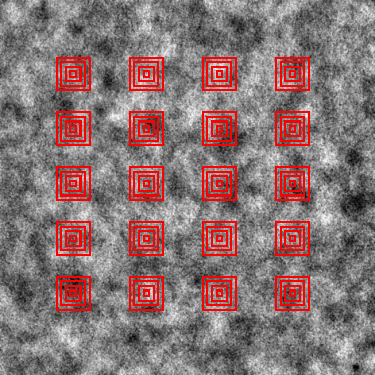
\includegraphics[width=0.4\textwidth]{Figures/fig-7.pdf}
		\caption[GNF calculations]
		{Calculation of the standard deviation of the average pixel intensity, $\Delta I$, at different length scales. Density fluctuations are quantified by the standard deviation of the average pixel intensity over time in subsystems of increasing sizes, indicated by the sequences of red squares. Results from twenty different subsystems of the same size evenly distributed in the field of view are then averaged to yield $\Delta I$ for the given subsystem size.}
		\label{GNF-calculation}
	\end{center}
\end{figure}


\section{Image analysis} \label{appendix-IA}
\subsection{Density fluctuations} \label{sec:GNF-calculations}

\subsubsection{Pixel intensity and bacterial number}
In Fig.~\ref{fig:experiment}d, we show that under the same illumination and imaging condition, bacterial density and the average pixel intensity follow approximately a linear relation, which can be expressed as follows:
\begin{equation}
\label{eq:phi-I-relation}
\phi = a + bI,
\end{equation}
where $\phi$ is the volume fraction of bacterial suspensions, $I$ is the average pixel intensity, $a$ and $b$ are constants at the fixed illumination and imaging condition. The number of bacteria in a given subsystem of side length $l$ and thickness $d$ can be calculated as
\begin{equation}
\label{eq:n}
N = \frac{l^2d}{V_b} \phi = \frac{l^2d}{V_b} (a+bI),
\end{equation}
where $V_b$ is the volume of a single bacterium. $d \approx 6$ $\mu$m is the depth of the field of microscopy, which is fixed in our experiments. Thus, the number of bacteria in the subsystem $N$ is proportional to $l^2 \phi$. Taking the standard deviation of both sides of Eq.~\ref{eq:n}, we obtain
\begin{equation}
\label{intensity-number}
\Delta N = \frac{l^2 d}{V_b}|b|\Delta I,
\end{equation}
where $\Delta N$ is the standard deviation of the bacterial number in the subsystem over time and $\Delta I$ is the standard deviation of the average pixel intensity of the subsystem over time. Since $d|b|/V_b$ is a constant independent of subsystem sizes and bacterial volume fractions, $\Delta N$ is linearly proportional to $l^2\Delta I$. Because any constant in front of $\Delta N$ would not affect either the scaling relation or the relative magnitude of density fluctuations at different $\phi$, we simply take $l^2\Delta I$ as $\Delta N$ in our study.

%%%%%%%%

\begin{figure}[t]
	\begin{center}
		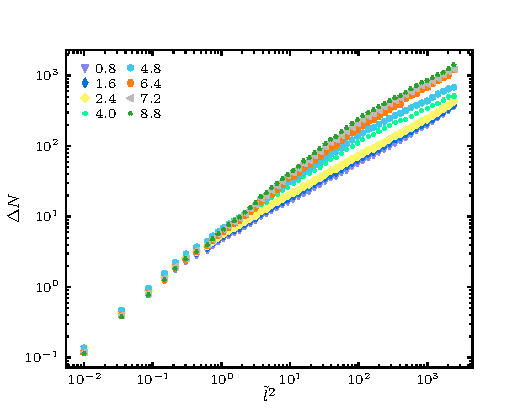
\includegraphics[width=0.47\textwidth]{Figures/fig-8.pdf}
		\caption[Density autocorrelation]
		{Calibration of the standard deviation of bacterial number $\Delta N \sim l^2\Delta I$ at different volume fractions $\phi$. $\Delta N$ versus the dimensionless subsystem size $\tilde{l}^2 = l^2/l_b^2$ for bacterial suspensions at different $\phi$. The images are taking under the same illumination with the same imaging condition.
		}
		\label{fig:same-conditions}
	\end{center}
\end{figure}

\subsubsection{Density fluctuations at different length scales}

Based on the linear relation between $\Delta N$ and $\Delta I$, we calculate the density fluctuations at different length scales. We first crop square-shape subsystems of increasing sizes, as shown in Fig.~\ref{GNF-calculation}. For each subsystem size $l$, the standard deviation of the average pixel intensity of the subsystem is calculated over 50 frames (1.67 s or 8.35$\tau_b$), which is longer than the saturated density correlation time of $4\tau_b = 0.8$ s (Fig.~\ref{fig:spatiotemporal-correlations}f). To improve statistics, we choose 20 subsystems of the same size evenly distributed in the field of view and obtain a spatial average of the temporal standard deviation of the average pixel intensity $\Delta I$ (Fig.~\ref{GNF-calculation}). This averaged $\Delta I$ is then multiplied by $l^2$ to give the number density fluctuations $\Delta N$ at the length scale $l$. Note that a second method has also been proposed for calculating number fluctuations, where the standard deviation of particle numbers is computed first spatially over different locations in a single time frame and is then averaged over time of different frames \cite{Aranson2008}.  Although the two methods lead to the same results when spatial and temporal correlations are small compared with the system size and experiment duration \cite{Aranson2008}, the second method is subject to potential systematic errors in our study due to time-independent non-uniform light illumination and intrinsic stationary density variations in non-motile suspensions at $t=0$ in the kinetic measurements. Using the first method, any stable non-uniform light illumination or stationary non-uniform density variations would result in zero temporal standard deviations of $I$ and, therefore, would not affect our measurements of true density fluctuations of motile bacterial suspensions.


\subsubsection{Normalization of bacterial suspensions of different volume fractions}

Practically, to optimize image qualities, we adjust the exposure time of imaging for suspensions of different $\phi$. Exposure times affect the proportional constant $b$ in Eq.~\ref{eq:phi-I-relation}, which introduces a $\phi$-dependent linear constant $b(\phi)$ in Eq.~\ref{eq:n}. Although $b(\phi)$ does not affect the scaling exponent of density fluctuations $\alpha$, it modifies the relative magnitude of $\Delta N$ at different $\phi$. In order to compare the magnitude of density fluctuations at different $\phi$,  we further calibrate and normalize $\Delta I$ for different $\phi$. Specifically, as the calibration, we take videos of bacterial suspensions at different $\phi$ under the exact same imaging condition with fixed illumination light intensity, condenser position, optical filters and all the camera settings such as the exposure time and the dynamic range. The calibration results are shown in Fig.~\ref{fig:same-conditions}, where $\Delta N \sim l^2 \Delta I$ at different $\phi$ collapse at small length scales. The calibration results show that we can normalize $l^2 \Delta I$ of different exposure times by its value at a fixed small length scale. We choose the small scale at $l = 0.3l_b$ in our study. Since $l^2 \Delta I$ at different $\phi$ shows the same slope at small $l$, choosing any other small lengths between $0.1l_b$ and $0.5l_b$ would lead to quantitatively the same results. The normalized density fluctuations show not only the correct scaling exponents but also the right relative magnitudes at different $\phi$.


\subsection{Particle image velocimetry (PIV)} \label{appendix-IA-PIV}

Two-dimensional in-plane velocity fields are extracted by Particle Image Velocimetry (PIV) analysis using the openPIV package in Python \cite{Liberzon2020}. We fix the box size to be 16.5 $\mu$m, which is larger than the size of a single bacterial body but smaller than the velocity correlation length. A step size of the half of the box size with $dx = 8.25$ $\mu$m is used by convention, which sets the spatial resolution of the velocity fields.

\subsection{Energy spectra} \label{appendix-IA-ES}
The energy spectra of bacterial suspensions are calculated as follows. First, we apply the built-in Fast Fourier Transform (FFT) function of Python \texttt{numpy.fft} package to convert the discrete velocity field $\bm{v}(\bm{r}) = [v_x(x,y), v_y(x,y)]$ obtained from PIV to the velocity field in the momentum space $\bm{v_k}(\bm{k}) = [u_k(k_x,k_y),v_k(k_x,k_y)]$. Note that to compensate the difference between FFT and the continuous Fourier transform, we time the $k$-space velocity from FFT by the square of the spatial spacing of the discrete $\bm{v}(\bm{r})$, $dx^2 = 68.1$ $\mu$m$^2$, in order to obtain $\bm{v_k}(\bm{k})$. The point-wise kinetic energy density in the $k$-space is then computed as
\begin{multline}
	E(k_x, k_y) = \\
	\frac{1}{2A}\langle u_k(k_x, k_y)u^*_k(k_x, k_y)+v_k(k_x, k_y)v_k^*(k_x, k_y)\rangle
\end{multline}
where $A$ is the total area of the field of view and $^*$ denotes the complex conjugate. $\langle\cdot\rangle$ denotes an average over multiple images from different times. Finally, the energy spectrum $E(k)$ is obtained by summing up $E(k_x,k_y)$ at a constant $k=(k_x^2+k_y^2)^{1/2}$. The approach is mathematically equivalent to the calculation of $E(k)$ from the Fourier transform of the two-point velocity correlation function $\langle \bm{v}(\bm{r_0}) \cdot \bm{v}(\bm{r_0}+\bm{r})) \rangle$.


\begin{figure}[t]
	\begin{center}
		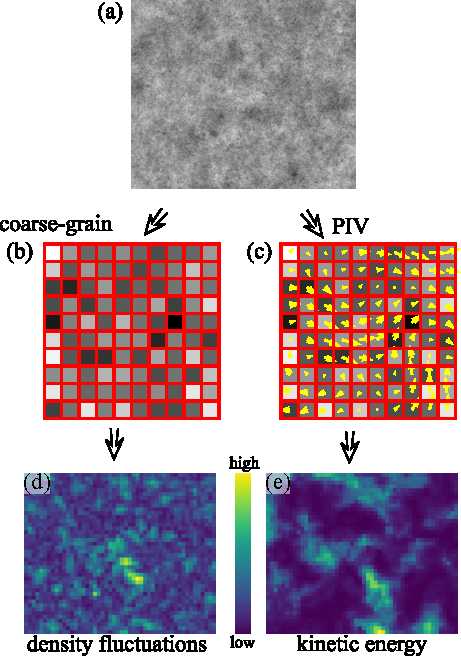
\includegraphics[width=0.46\textwidth]{Figures/fig-9.pdf}
		\caption[Density autocorrelation]
		{
			Diagram showing the procedure to calculate the correlation between local density fluctuations and kinetic energies. (a) The raw image of a bacterial suspension at a given time $t$. (b) The coarse-grained image with a pixel size of $l=2.75l_b$. (c) The velocity field from PIV. (d) The field of local density fluctuations, obtained by calculating the standard deviation of the intensity of coarsen-grained pixels shown in (b) over a short time interval. (e) The field of local kinetic energy, obtained by calculating $E = \bm{v}^2/2$ from the velocity field shown in (c).
 		}
		\label{fig:coupling-calculation}
	\end{center}
\end{figure}

\subsection{Correlation of local density fluctuations and kinetic energies} \label{appendix-IA-localcorrelation}

To calculate local temporal density fluctuations, we need to approximate instantaneous intensity variations. On the one hand, the time interval for calculating the intensity difference between two frames needs to be smaller than the density correlation time ($4\tau_b = 0.8$ s) in order to satisfy the instantaneous approximation. On the other hand, the time interval should be sufficiently long to suppress the influence of random fluctuations of image intensities in adjacent frames. In our study, we choose 0.3 s (10 frames) for the local density fluctuation calculation. We do not expect the results to be much different when varying this number from 0.17 to 0.6 s.

To calculate the local density variations at the length scale of $l = 2.75l_b$ and time $t$, we take 10 consecutive frames following the frame at $t$. All the 10 frames are first coarse-grained by averaging the intensity of pixels in square windows of size $2.75l_b \times 2.75l_b$ into single coarse-grained pixels (Fig.~\ref{fig:coupling-calculation}b). We then take the temporal standard deviation of the coarse-grained pixel intensity over the 10 frames at different positions to obtain a field of density fluctuations at $t$, $\delta N(\bm{r},t)$, as shown in Fig.~\ref{fig:coupling-calculation}d. The same approach has also been used to calculate the field of instantaneous density fluctuations in the transient state shown in Fig.~\ref{fig:GNF-energy-spectra-correlation-transient}a.

Independently, the PIV algorithm is also applied on the original images of the first two frames to obtain the velocity field at time $t$, $\bm{v}(\bm{r},t)$ (Fig.~\ref{fig:coupling-calculation}c). Since the step size of the PIV analysis is also at $2.75l_b$, the velocity field has the same dimensions as the coarse-grained density fluctuation field obtained above. The local kinetic energy can then be calculated as $E(\bm{r},t)=|\bm{v}(\bm{r},t)|^2/2$ (Fig.~\ref{fig:coupling-calculation}e). Finally, the normalized correlation between $\delta N(\bm{r},t)$ and $E(\bm{r},t)$ is computed as
\begin{equation}
C_s = \frac{\langle(\Delta N-\overline{\Delta N})(E-\overline{E})\rangle}{\sigma_{\Delta N}\sigma_{E}},
\end{equation}
where $\bar A$ indicates the mean of variable $A$, $\sigma_A$ indicates the standard deviation of $A$, and $\langle A \rangle$ denotes the average of $A$ over all the positions. The correlation quantifies the spatial similarity between $\delta N$ and $E$, which ranges between $-1$ to 1. Finally, the correlation $C$ shown in Fig.~\ref{fig:GNF-energy-spectra-correlation}b is
calculated by averaging $C_s$ over 1000 frames.


\subsection{Density fluctuations in the transient state} \label{appendix-IA-transient}

Density fluctuations in the transient state towards active turbulence is calculated using the same method as that in the steady state. Specifically, the procedure described in Sec.~\ref{sec:GNF-calculations} is applied at time $t$ over a time interval $\Delta t$ during the transition towards active turbulence. We choose $\Delta t = 1.7$ s (50 frames), which is longer than the density correlation time ($4\tau_b = 0.8$ s) but is significantly smaller than the time of the entire transition ($\sim 60$ s or 1800 frames) for a sufficient temporal resolution.

\bibliographystyle{prx_bib}
\bibliography{correlation}

\end{document}
